% move all configuration stuff into one file so we can focus on the content
\documentclass[aspectratio=169,hyperref={pdfpagelabels=false,colorlinks=true,linkcolor=white,urlcolor=lightblue},xcolor={table},t]{beamer}

%%%%%%%%%%%%%%%%%%%%%%%%%%%%%%%%%%%%%%%%%%%%%%%%%%%%%%%%%%%%%%%%%%%%%%%%%%%%%%%%%%
%%%%%%%%%%%%%%%%%%%%%%%%%%%%%%%%%%%%%%%%%%%%%%%%%%%%%%%%%%%%%%%%%%%%%%%%%%%%%%%%%%
% packages
\usepackage{pict2e}
\usepackage{epic}
\usepackage{amsmath,amsfonts,amssymb}
\usepackage{units}
\usepackage{fancybox}
\usepackage[absolute,overlay]{textpos} 
%\usepackage[table]{xcolor}
\usepackage{animate}
\usepackage{gensymb}
%\usepackage{graphicx}
%\usepackage{longtable}
\usepackage{multirow}
\usepackage{silence}
\usepackage{tikz}
\usepackage[backend=bibtex,style=ieee]{biblatex}
\AtEveryCitekey{\iffootnote{\tiny}{}}
%\addbibresource{include/references}



% fontsize
\let\Tiny=\tiny

%%%%%%%%%%%%%%%%%%%%%%%%%%%%%%%%%%%%%%%%%%%%%%%%%%%%%%%%%%%%%%%%%%%%%%%%%%%%%%%%%%
%%%%%%%%%%%%%%%%%%%%%%%%%%%%%%%%%%%%%%%%%%%%%%%%%%%%%%%%%%%%%%%%%%%%%%%%%%%%%%%%%%
% warnings
\pdfsuppresswarningpagegroup=1
\WarningFilter{biblatex}{Patching footnotes failed}
\WarningFilter{latexfont}{Font shape}
\WarningFilter{latexfont}{Some font shapes}
\WarningFilter{gensymb}{Not defining}


%%%%%%%%%%%%%%%%%%%%%%%%%%%%%%%%%%%%%%%%%%%%%%%%%%%%%%%%%%%%%%%%%%%%%%%%%%%%%%%%%%
%%%%%%%%%%%%%%%%%%%%%%%%%%%%%%%%%%%%%%%%%%%%%%%%%%%%%%%%%%%%%%%%%%%%%%%%%%%%%%%%%%
% theme & layout
\usetheme{Frankfurt}
\useinnertheme{rectangles}


%%%%%%%%%%%%%%%%%%%%%%%%%%%%%%%%%%%%%%%%%%%%%%%%%%%%%%%%%%%%%%%%%%%%%%%%%%%%%%%%%%
\setbeamertemplate{frametitle}[default][colsep=-4bp,rounded=false,shadow=false]
\setbeamertemplate{frametitle}
{%
    \nointerlineskip%
    %\vskip-0.5ex
    \begin{beamercolorbox}[wd=\paperwidth,ht=3.5ex,dp=0.6ex]{frametitle}
        \hspace*{1.3ex}\insertframetitle%
        
        \hspace*{1.3ex}\small\insertframesubtitle%
    \end{beamercolorbox}%
    \begin{textblock*}{100mm}(13.75cm,1cm)
        
\includegraphics[height=.4cm,keepaspectratio]{../shared/Logo_GTCMT_white}
    \end{textblock*}
}


%%%%%%%%%%%%%%%%%%%%%%%%%%%%%%%%%%%%%%%%%%%%%%%%%%%%%%%%%%%%%%%%%%%%%%%%%%%%%%%%%%
\setbeamertemplate{title page}[default][colsep=-4bp,rounded=false,shadow=false]
\setbeamertemplate{title page}
{
    %\begin{textblock*}{100mm}(15cm,.51cm)
            %\href{https://github.com/alexanderlerch/ACA-Slides/blob/2nd_edition/\jobname.pdf}{\includegraphics[height=.5cm,keepaspectratio]{graph/Logo_github}}\hspace*{2ex}
    %\end{textblock*}
    %\begin{textblock*}{100mm}(15cm,1.3cm)
            %\href{\IEEELink}{\includegraphics[height=.5cm,keepaspectratio]{graph/icon/book}}\hspace*{2ex}
    %\end{textblock*}
    \vskip-10ex
    \begin{beamercolorbox}[wd=\paperwidth,ht=.7\paperheight,dp=0.6ex]{frametitle} %35ex
        %\begin{flushright}
            %\href{http://www.gtcmt.gatech.edu}{
\includegraphics[height=.8cm,keepaspectratio]{graph/Logo_GTCMT_black}}\hspace*{2ex}
        %\end{flushright}
        
        \hspace*{1.8ex}\LARGE\inserttitle%
        
        \vspace*{.5ex}
        
        \hspace*{1.3ex}\small\insertsubtitle%
        
        \vspace*{.5ex}
    \end{beamercolorbox}%
    \nointerlineskip%
    \begin{beamercolorbox}[wd=\paperwidth,ht=.4\paperheight,dp=0.6ex]{page number in head/foot}
        %\vspace*{-.5ex}
        \hspace*{1.7ex}\small\insertauthor%
        
        %\hspace*{1.7ex}\small }%
        
        \vspace*{12ex}
        \vfill
        \begin{flushright}
            \href{http://www.gtcmt.gatech.edu}{
\includegraphics[height=.5cm,keepaspectratio]{../shared/Logo_GTCMT_black}}\hspace*{2ex}
        \end{flushright}
    \end{beamercolorbox}%
}


%%%%%%%%%%%%%%%%%%%%%%%%%%%%%%%%%%%%%%%%%%%%%%%%%%%%%%%%%%%%%%%%%%%%%%%%%%%%%%%%%%
%\makeatother
\setbeamertemplate{footline}
{
  \leavevmode%
  \hbox{%
  \begin{beamercolorbox}[wd=.5\paperwidth,ht=2.25ex,dp=1ex,left,leftskip=1ex]{page number in head/foot}%
    \insertsubtitle
  \end{beamercolorbox}%
  \begin{beamercolorbox}[wd=.5\paperwidth,ht=2.25ex,dp=1ex,right,rightskip=1ex]{page number in head/foot}%
    \hfill
    \insertframenumber{} / \inserttotalframenumber
  \end{beamercolorbox}}%
  \vskip0pt%
}
%\makeatletter


%%%%%%%%%%%%%%%%%%%%%%%%%%%%%%%%%%%%%%%%%%%%%%%%%%%%%%%%%%%%%%%%%%%%%%%%%%%%%%%%%%
\beamertemplatenavigationsymbolsempty
\setbeamertemplate{navigation symbols}{}
\setbeamertemplate{blocks}[default]%[rounded=false,shadow=false]
\setbeamertemplate{itemize item}[square]
\setbeamertemplate{itemize subitem}[circle]
\setbeamertemplate{itemize subsubitem}[triangle]
\setbeamertemplate{enumerate item}[square]
\setbeamertemplate{enumerate subitem}[circle]
\setbeamertemplate{enumerate subsubitem}[circle]


%%%%%%%%%%%%%%%%%%%%%%%%%%%%%%%%%%%%%%%%%%%%%%%%%%%%%%%%%%%%%%%%%%%%%%%%%%%%%%%%%%
% colors
\setbeamercolor{structure}{fg=darkgray}
\setbeamercovered{transparent} %invisible
\setbeamercolor{bibliography entry author}{fg=black}
\setbeamercolor*{bibliography entry title}{fg=black}
\setbeamercolor*{bibliography entry note}{fg=black}
\setbeamercolor{frametitle}{fg=black}
\setbeamercolor{title}{fg=white}
\setbeamercolor{subtitle}{fg=white}
\setbeamercolor{frametitle}{fg=white}
\setbeamercolor{framesubtitle}{fg=white}
\setbeamercolor{mini frame}{fg=white, bg=black}
\setbeamercolor{section in head/foot}{fg=white, bg=darkgray}
\setbeamercolor{page number in head/foot}{fg=black, bg=gtgold}
\setbeamercolor{item projected}{fg=white, bg=black}

%---------------------------------------------------------------------------------

%%%%%%%%%%%%%%%%%%%%%%%%%%%%%%%%%%%%%%%%%%%%%%%%%%%%%%%%%%%%%%%%%%%%%%%%%%%%%%%%%%
%%%%%%%%%%%%%%%%%%%%%%%%%%%%%%%%%%%%%%%%%%%%%%%%%%%%%%%%%%%%%%%%%%%%%%%%%%%%%%%%%%
% title information
\title[]{MUSI6202: Digital Signal Processing for Music}   
\author[alexander lerch]{alexander lerch} 
%\institute{~}
%\date[Alexander Lerch]{}
%\titlegraphic{\vspace{-16mm}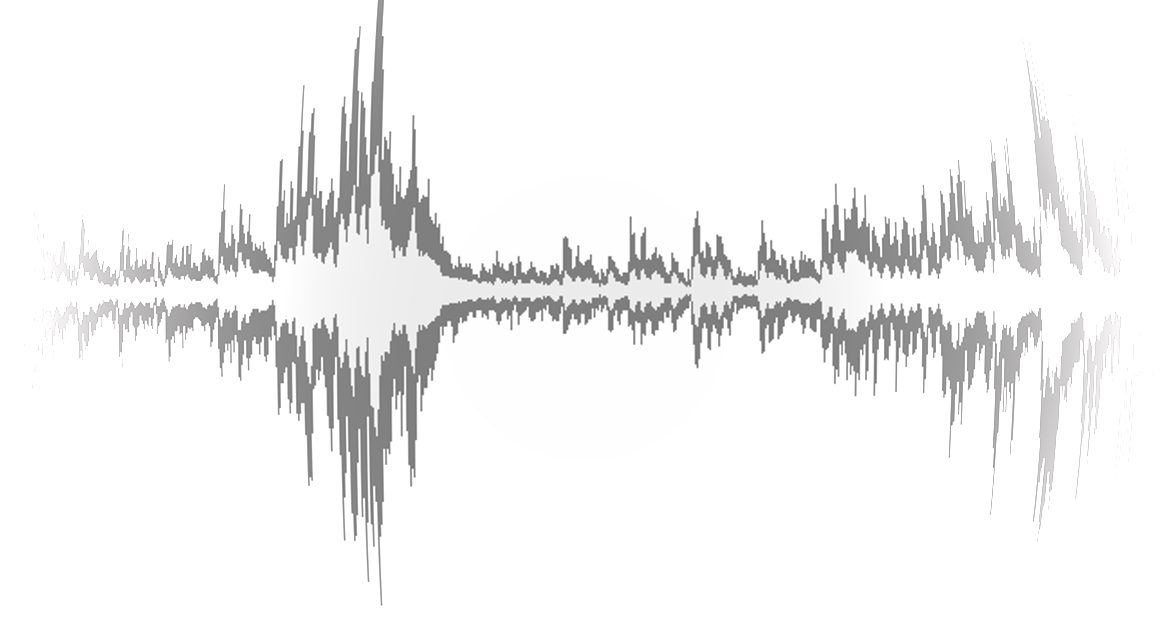
\includegraphics[width=\textwidth,height=3cm]{title}}

%%%%%%%%%%%%%%%%%%%%%%%%%%%%%%%%%%%%%%%%%%%%%%%%%%%%%%%%%%%%%%%%%%%%%%%%%%%%%%%%%%
%%%%%%%%%%%%%%%%%%%%%%%%%%%%%%%%%%%%%%%%%%%%%%%%%%%%%%%%%%%%%%%%%%%%%%%%%%%%%%%%%%
% colors
\definecolor{gtgold}{rgb}{.914, .664, 0} %0e7eed {rgb}{0.88,0.66,1,0.06} [234, 170, 0]/256 %96caff
\definecolor{darkgray}{rgb}{.15, .15, .15}
\definecolor{lightblue}{HTML}{0e7eed}
\definecolor{highlight}{rgb}{0, 0, 1} %_less!40

%%%%%%%%%%%%%%%%%%%%%%%%%%%%%%%%%%%%%%%%%%%%%%%%%%%%%%%%%%%%%%%%%%%%%%%%%%%%%%%%%%
%%%%%%%%%%%%%%%%%%%%%%%%%%%%%%%%%%%%%%%%%%%%%%%%%%%%%%%%%%%%%%%%%%%%%%%%%%%%%%%%%%
% relative paths
\graphicspath{{../graph/}}


%%%%%%%%%%%%%%%%%%%%%%%%%%%%%%%%%%%%%%%%%%%%%%%%%%%%%%%%%%%%%%%%%%%%%%%%%%%%%%%%%%
%%%%%%%%%%%%%%%%%%%%%%%%%%%%%%%%%%%%%%%%%%%%%%%%%%%%%%%%%%%%%%%%%%%%%%%%%%%%%%%%%%
% units
\setlength{\unitlength}{1mm}

%%%%%%%%%%%%%%%%%%%%%%%%%%%%%%%%%%%%%%%%%%%%%%%%%%%%%%%%%%%%%%%%%%%%%%%%%%%%%%%%%%
%%%%%%%%%%%%%%%%%%%%%%%%%%%%%%%%%%%%%%%%%%%%%%%%%%%%%%%%%%%%%%%%%%%%%%%%%%%%%%%%%%
% math
\DeclareMathOperator*{\argmax}{argmax}
\DeclareMathOperator*{\argmin}{argmin}
\DeclareMathOperator*{\atan}{atan}
\DeclareMathOperator*{\arcsinh}{arcsinh}
\DeclareMathOperator*{\sign}{sign}
\DeclareMathOperator*{\tcdf}{tcdf}
\DeclareMathOperator*{\si}{sinc}
\DeclareMathOperator*{\princarg}{princarg}
\DeclareMathOperator*{\arccosh}{arccosh}
\DeclareMathOperator*{\hwr}{HWR}
\DeclareMathOperator*{\flip}{flip}
\DeclareMathOperator*{\sinc}{sinc}
\DeclareMathOperator*{\floor}{floor}
\newcommand{\e}{{e}}
\newcommand{\jom}{\mathrm{j}\omega}
\newcommand{\jOm}{\mathrm{j}\Omega}
\newcommand   {\mat}[1]    		{\boldsymbol{\uppercase{#1}}}		%bold
\renewcommand {\vec}[1]    		{\boldsymbol{\lowercase{#1}}}		%bold

%%%%%%%%%%%%%%%%%%%%%%%%%%%%%%%%%%%%%%%%%%%%%%%%%%%%%%%%%%%%%%%%%%%%%%%%%%%%%%%%%%
%%%%%%%%%%%%%%%%%%%%%%%%%%%%%%%%%%%%%%%%%%%%%%%%%%%%%%%%%%%%%%%%%%%%%%%%%%%%%%%%%%
% media9
\newcommand{\includeaudio}[1]{
\href{run:audio/#1.mp3}{
\includegraphics[width=5mm, height=5mm]{graph/SpeakerIcon}}}

\newcommand{\includeanimation}[4]{{\begin{center}
                        \animategraphics[autoplay,loop,scale=.7]{#4}{animation/#1-}{#2}{#3}        
                        \end{center}
                        \addreference{matlab source: \href{https://github.com/alexanderlerch/ACA-Plots/blob/master/matlab/animate#1.m}{matlab/animate#1.m}}}
                        \inserticon{video}}
                        
%%%%%%%%%%%%%%%%%%%%%%%%%%%%%%%%%%%%%%%%%%%%%%%%%%%%%%%%%%%%%%%%%%%%%%%%%%%%%%%%%%
%%%%%%%%%%%%%%%%%%%%%%%%%%%%%%%%%%%%%%%%%%%%%%%%%%%%%%%%%%%%%%%%%%%%%%%%%%%%%%%%%%
% other commands
\newcommand{\question}[1]{%\vspace{-4mm}
                          \setbeamercovered{invisible}
                          \begin{columns}[T]
                            \column{.9\textwidth}
                                \textbf{#1}
                            \column{.1\textwidth}
                                \vspace{-8mm}
                                \begin{flushright}
                                     
\includegraphics[width=.9\columnwidth]{graph/question_mark}
                                \end{flushright}
                                \vspace{6mm}
                          \end{columns}\pause\vspace{-12mm}}

\newcommand{\toremember}[1]{
                        \inserticon{lightbulb}
                        }

\newcommand{\matlabexercise}[1]{%\vspace{-4mm}
                          \setbeamercovered{invisible}
                          \begin{columns}[T]
                            \column{.8\textwidth}
                                \textbf{matlab exercise}: #1
                            \column{.2\textwidth}
                                \begin{flushright}
                                     \includegraphics[scale=.5]{graph/logo_matlab}
                                \end{flushright}
                                %\vspace{6mm}
                          \end{columns}}

\newcommand{\addreference}[1]{  
                  
                    \begin{textblock*}{\baselineskip }(.98\paperwidth,.5\textheight) %(1.15\textwidth,.4\textheight)
                         \begin{minipage}[b][.5\paperheight][b]{1cm}%
                            \vfill%
                             \rotatebox{90}{\tiny {#1}}
                        \end{minipage}
                   \end{textblock*}
                    }
                    
\newcommand{\figwithmatlab}[1]{
                    \begin{figure}
                        \centering
                        \includegraphics[scale=.7]{#1}
                        %\label{fig:#1}
                    \end{figure}
                    
                    \addreference{matlab source: \href{https://github.com/alexanderlerch/MUSI-6202/blob/main/matlab/plot#1.m}{plot#1.m}}}
\newcommand{\figwithref}[2]{
                    \begin{figure}
                        \centering
                        \includegraphics[scale=.7]{#1}
                        \label{fig:#1}
                    \end{figure}
                    
                    \addreference{#2}}  
                                    
\newcommand{\inserticon}[1]{
                    \begin{textblock*}{100mm}(14.5cm,7.5cm)
                        \includegraphics[height=.8cm,keepaspectratio]{graph/#1}
                    \end{textblock*}}            

%%%%%%%%%%%%%%%%%%%%%%%%%%%%%%%%%%%%%%%%%%%%%%%%%%%%%%%%%%%%%%%%%%%%%%%%%%%%%%%%%%
%%%%%%%%%%%%%%%%%%%%%%%%%%%%%%%%%%%%%%%%%%%%%%%%%%%%%%%%%%%%%%%%%%%%%%%%%%%%%%%%%%
% counters
\newcounter{i}
\newcounter{j}
\newcounter{iXOffset}
\newcounter{iYOffset}
\newcounter{iXBlockSize}
\newcounter{iYBlockSize}
\newcounter{iYBlockSizeDiv2}
\newcounter{iXBlockSizeDiv2}
\newcounter{iDistance}

\newcommand{\IEEELink}{https://ieeexplore.ieee.org/servlet/opac?bknumber=9965970}

\addbibresource{../shared/references}



\subtitle{Part 16: z-transform}

%%%%%%%%%%%%%%%%%%%%%%%%%%%%%%%%%%%%%%%%%%%%%%%%%%%%%%%%%%%%%%%%%%%%%%%%%%%%
\begin{document}
    % generate title page
	\title[]{Digital Signal Processing for Music}   
\author[alexander lerch]{alexander lerch} 
%\institute{~}
%\date[Alexander Lerch]{}
\titlegraphic{\vspace{-16mm}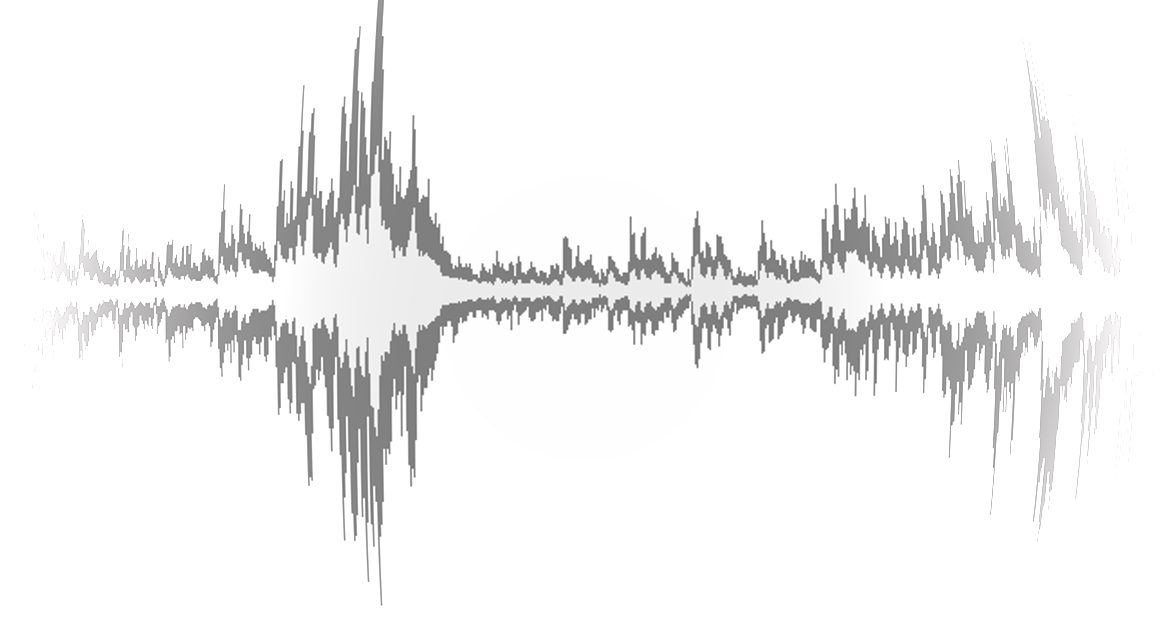
\includegraphics[width=\textwidth,height=3cm]{title}}


\begin{frame}
    \titlepage
    %\vspace{-5mm}
    \begin{flushright}
        \href{http://www.gtcmt.gatech.edu}{
\includegraphics[height=.8cm,keepaspectratio]{../shared/Logo_GTCMT_black}}
    \end{flushright}
\end{frame}


\section[intro]{introduction}
	\begin{frame}{z-transform}{introduction}
        the z-transform is
        \begin{itemize}
            \item   a generalization of DFT,
            \smallskip
            \item   widely used in DSP as analysis tool,
            \smallskip
            \item   a useful tool to characterize systems (also recursive systems!),
            \smallskip
            \item   a useful tool to check for system stability and causality,
            \smallskip
            \item   the discrete-time counterpart of the Laplace transform.
        \end{itemize}
	\end{frame}

\section{z-transform}
	\begin{frame}{z-transform}{definition}
        \begin{equation*}
            X(z) = \sum\limits_{i=-\infty}^{\infty}{x(i)z^{-i}},\quad z\in \mathfrak{C}
        \end{equation*}
        \begin{itemize}
            \item<2->   $X(z)$: complex function of a complex number
            \bigskip
            \item<3->   compare Fourier transform $X(\jom)$: complex function of real-valued $\omega$
        \end{itemize}
        \only<3->{
        \begin{equation*}
            X(\jom) = \sum\limits_{i=-\infty}^{\infty}{x(i)e^{-\jom i}}
            \Rightarrow X(\jom) = X(z) \text{ at }z=e^{\jom}
        \end{equation*}
        }
	\end{frame}
	\begin{frame}{z-transform}{zplane}
        \vspace{-5mm}
        \begin{columns}
            \column{.5\linewidth}
                \begin{itemize}
                    \item $X(z)$ defined on complex plane
                    \item   $X(\jom)$ defined on unit circle
                    \bigskip 
                    \item<3-> observation: $X(\jom)$ is periodic with $2\pi$
                \end{itemize}
            \column{.5\linewidth}
                \figwithmatlab{ZplaneIntro}
        \end{columns}
	\end{frame}
	\begin{frame}{z-transform}{trivial examples}
        \figwithmatlab{ZplaneExample}
        
        \question{what is the magnitude for $X(z) = 1/(z-0.5)$}
        
        same as $1/z$ but shifted on the x-axis.
        
	\end{frame}
	\begin{frame}{z-transform}{system description}
        Fourier transform and z-transform have largely similar properties, most importantly
        \begin{itemize}
            \item   \textbf{linearity}
                \begin{eqnarray*}
                    y(i) = c_1 x_1(i) + c_2 x_2(i) &\Rightarrow& Y(\jom) = c_1 X_1(\jom) + c_2 X_2(\jom)\\
                     &\Rightarrow& Y(z) = c_1 X_1(z) + c_2 X_2(z)
                \end{eqnarray*}
            \smallskip
            \item   \textbf{time shift}
                \begin{eqnarray*}
                    y(i) = x(i-n) &\Rightarrow& Y(\jom) = e^{-\jom n} X(\jom) \\
                     &\Rightarrow& Y(z) =  z^{-n} X(z)
                \end{eqnarray*}
        \end{itemize}
        
	\end{frame}

		\begin{frame}{z-transform}{biquad: difference equation}
        \vspace{-3mm}
        \setbeamercovered{invisible}
        \setlength{\unitlength}{1pt}
	        \begin{figure}[!hbt]
				\begin{center}
	            \begin{picture}(180,80)

					%%%%%%%%%%%%%%%%%%%%%%%%%%%%%%%%%%%%%%%%%%%%%%%%%%%%%%%
					%FIR	
	                %boxes
	                \put(22,47){\framebox(16,14){\footnotesize{$z^{-1}$}}}
	                \put(22,11){\framebox(16,14){\footnotesize{$z^{-1}$}}}
	
	                %lines horizontal
	                \put(19,72){\vector(1,0){37}}
	                \put(62,72){\vector(1,0){21}}
	                \put(89,72){\vector(1,0){28}}
	                
	                \put(30,38.5){\vector(1,0){26}}
	                \put(62,38.5){\vector(1,0){21.5}}
	                
	                \put(30,2.5){\vector(1,0){26}}
	                \put(62,2.5){\line(1,0){24}}
	
	                %lines vertical
	                \put(86,42){\vector(0,1){27.5}}
	                \put(30,47){\line(0,-1){9}}
	                \put(30,72){\vector(0,-1){10.5}}

	                \put(86,2.5){\vector(0,1){32.5}}
	                \put(30,11){\line(0,-1){8.5}}
	                \put(30,39){\vector(0,-1){13}}
	                
	                %circles
	                \put(55,69.5){$\otimes$}
	                \put(82,69.5){$\oplus$} 
	                \put(55,36){$\otimes$}

	                \put(82,36){$\oplus$} 
	                \put(55,0){$\otimes$}
	                
	                \put(30,72){\circle*{2}}
	                \put(30,38.5){\circle*{2}}
	
	                %text
	                \put(59,76){\footnotesize{\shortstack[c]{$b_0$}}}
	                \put(59,42.5){\footnotesize{\shortstack[c]{$b_1$}}}
	                \put(59,6.5){\footnotesize{\shortstack[c]{$b_2$}}}
	
	                \put(12,75){\footnotesize{\shortstack[c]{x(n)}}}
	                %\put(93,75){\footnotesize{\shortstack[c]{y(n)}}}


					%%%%%%%%%%%%%%%%%%%%%%%%%%%%%%%%%%%%%%%%%%%%%%%%%%%%%%%
					%IIR	
	                %boxes
	                \put(168,47){\framebox(16,14){\footnotesize{$z^{-1}$}}}
	                \put(168,11){\framebox(16,14){\footnotesize{$z^{-1}$}}}
	
	                %lines horizontal
	                %\put(89,72){\vector(1,0){37}}
	                %\put(152,72){\vector(1,0){21}}
	                \put(123,72){\vector(1,0){67}}
	                
	                \put(176,38.5){\vector(-1,0){24}}
	                \put(146,38.5){\vector(-1,0){23.5}}
	                
	                \put(176,2.5){\vector(-1,0){24}}
	                \put(146,2.5){\line(-1,0){26}}
	
	                %lines vertical
	                \put(120,42){\vector(0,1){27.5}}
	                \put(176,47){\line(0,-1){9}}
	                \put(176,72){\vector(0,-1){10.5}}

	                \put(120,2.5){\vector(0,1){32.5}}
	                \put(176,11){\line(0,-1){8.5}}
	                \put(176,39){\vector(0,-1){13}}
	                
	                %circles
	                %\put(145,69.5){$\otimes$}
	                \put(116,69.5){$\oplus$} 
	                \put(145,36){$\otimes$}

	                \put(116,36){$\oplus$} 
	                \put(145,0){$\otimes$}
	                
	                \put(176,72){\circle*{2}}
	                \put(176,38.5){\circle*{2}}
	
	                %text
	                \put(149,42.5){\footnotesize{\shortstack[c]{$-a_1$}}}
	                \put(149,6.5){\footnotesize{\shortstack[c]{$-a_2$}}}
	
	                %\put(102,75){\footnotesize{\shortstack[c]{x(n)}}}
	                \put(183,75){\footnotesize{\shortstack[c]{y(n)}}}
	
	            \end{picture}
				\end{center}
	        \end{figure}
        	\pause
            \setlength{\unitlength}{1mm}
        	\begin{eqnarray*}
        		y(i) &=& \sum\limits_{j=0}^{2}{b_j x(i-j)} - \sum\limits_{k=1}^{2}{a_j y(i-j)}\nonumber\\
        		\pause
        		Y(z) &=& \sum\limits_{j=0}^{2}{b_j X(z) z^{-j}} - \sum\limits_{k=1}^{2}{a_j Y(z) z^{-j}}\nonumber\\
        		\pause
        		Y(z)\left(1+\sum\limits_{j=1}^{2}{a_j z^{-j}}\right) &=& X(z) \sum\limits_{j=0}^{2}{b_j z^{-j}}\nonumber   		
        	\end{eqnarray*}
 		\end{frame}

		\begin{frame}{biquad}{ transfer function}
			\begin{eqnarray*}
				H(z) &=& \frac{Y(z)}{X(z)}\nonumber\\
				\pause
					 &=& \frac{\sum\limits_{j=0}^{2}{b_j z^{-j}}}{1+\sum\limits_{j=1}^{2}{a_j z^{-j}}}\nonumber\\
				\pause
				     &=& \frac{b_0 + b_1\cdot z^{-1} + b_2\cdot z^{-2}}{1 + a_1\cdot z^{-1} + a_2\cdot z^{-2}}\nonumber\\
					 &=&\frac{\text{numerator polynomial}}{\text{denominator polynomial}}\nonumber
					 %&=&\frac{b_0 + b_1\cdot z^{-1} + b_2\cdot z^{-2}}{(1- z_{\infty 1}\cdot z^{-1})(1- z_{\infty 2}\cdot z^{-1})}\nonumber
			\end{eqnarray*}
 		\end{frame}
		\begin{frame}{biquad}{ poles and zeros}
			\begin{itemize}
				\item	numerator $\rightarrow 0$: zero
				\only<1>{\item	denominator  $\rightarrow 0$: pole}
				\only<2->{\item	\textcolor{gtgold}{denominator  $\rightarrow 0$: pole}}
                \only<5->{
                    \bigskip
                    \item   zeros and poles are a simplified way of visualizing filter properties in the zplane
                    }
			\end{itemize}
			\visible<3,4>{
				\begin{eqnarray*}
					1 + a_1\cdot z^{-1} + a_2\cdot z^{-2} &=& 0\nonumber\\
	%							z^2 + a_1\cdot z + a_2 &=& 0\nonumber
                    \pause
					\Longrightarrow z_{\infty1,2} &=& \frac{a_1}{2} \pm \frac{1}{2}\sqrt{a_1^2-4a_2}\nonumber
				\end{eqnarray*}
			}
		\end{frame}
		\begin{frame}{biquad}{zplane example}
            \figwithmatlab{BiquadZplane}
 		\end{frame}
		\begin{frame}{biquad}{ animation}
            \vspace{-5mm}
            \includeanimation{BiquadZplane}{01}{400}{10}
 		\end{frame}

		%\begin{frame}{filters}{z-transform}
            %\begin{equation*}
                %X(z) = \sum\limits_{i=-\infty}^\infty x(i)z^{-i}
            %\end{equation*}
            %\begin{equation*}
                %z = \Re\lbrace z \rbrace + \mathrm{j}\Im\lbrace z \rbrace
            %\end{equation*}
            %\pause
            %relation to Fourier transform:
             %\begin{equation*}
                %X(z)_{|z=e^{\jOm}} = X(\jOm) = \mathfrak{F}\lbrace x(i)\rbrace
            %\end{equation*}
 		%\end{frame}
        
    \section{characteristics}
		%\begin{frame}{z-transform}{convergence introduction}
            %\begin{equation*}
                %X(z) = \sum\limits_{i=-\infty}^\infty x(i)z^{-i}
            %\end{equation*}
            %is not defined for all z
            %
            %
            %\pause
            %example:
                %\begin{equation*}
                    %x(i) = \delta(i-n_0) \Rightarrow X(z) = \sum\limits_{i=-\infty}^\infty \delta(i-n_0)z^{-i} = z^{-n_0}
                %\end{equation*}
            %\begin{itemize}
                %\item<3->   does not exist for $z=0, n_0>0$
                %\item<3->   does not exist for $z=\infty, n_0<0$
            %\end{itemize}
		%\end{frame}
		%\begin{frame}{z-transform}{convergence of the z-transform 1/3}
            %\begin{itemize}
                %\item definition
                %\begin{footnotesize}
                %\begin{equation*}
                    %X(z) = \sum\limits_{i=-\infty}^\infty x(i)z^{-i}
                %\end{equation*}
                %\end{footnotesize}
                %\pause
                %\item   stability
                %\begin{footnotesize}
                 %\begin{equation*}
                    %|X(z)| = \left|\sum\limits_{i=-\infty}^\infty x(i)z^{-i}\right| \leq \sum\limits_{i=-\infty}^\infty |x(i)||z|^{-i} \leq \infty
                %\end{equation*}
                 %\end{footnotesize}
                   %\begin{enumerate}
                        %\item   right side: $\lim\limits_{N\rightarrow\infty}\sum\limits_{i=0}^N x(i)z^{-i}$ converges for $|z| > R_1$
                        %\pause
                        %\item   left side: $\lim\limits_{N\rightarrow\infty}\sum\limits_{i=-\infty}^{-1} x(i)z^{-i}=\lim\limits_{N\rightarrow\infty}\sum\limits_{n=1}^{N} x(-n)z^{n}$ converges for $|z| < R_2$
                    %\end{enumerate}
           %\end{itemize}
 		%\end{frame}
		%\begin{frame}{z-transform}{convergence of the z-transform 2/3}
            %\begin{equation*}
                %\text{Region of Convergence (ROC): } R_1\leq |z| \leq R_2
            %\end{equation*}
            %\pause
            %
            %\begin{itemize}
                %\item                 \textbf{observations}
                %\begin{itemize}
                    %\item   $R_1,R_2$ define circles
                    %\item   $R_1 > R_2$: z-transform does not exist
                    %\item   causality: $R_2 \rightarrow \infty$
                %\end{itemize}
                %\item   \textbf{properties}
                    %\begin{itemize}
                        %\item   ROC cannot contain poles, boundaries include poles (or are at $0, \infty$)
                        %\item   since we need $|H(\jOm)|$ to exist, $R_1 \leq 1$!
                    %\end{itemize}
            %\end{itemize}
 		%\end{frame}
		%\begin{frame}{filters}{convergence of the z-transform 3/3}
            %\begin{figure}
                %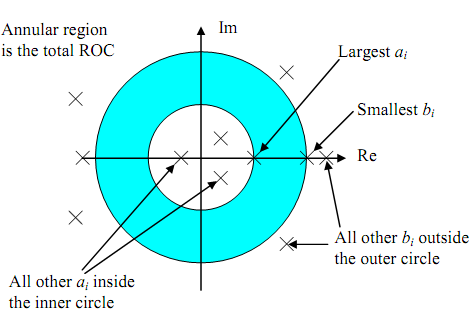
\includegraphics[scale=.8]{graph/ROC}
            %\end{figure}
 		%\end{frame}
		%\begin{frame}{filters}{convergence example}
            %example: damped sinusoidal $ h(i) = R^i e^{\jom iT}$
            %\begin{eqnarray*}
                %H(z) &=& \sum\limits_{n=0}^\infty  R^n e^{\jom nT}z^{-n}\\
                %&=& \sum\limits_{n=0}^\infty  \left(R e^{\jom T}z^{-1}\right)^n\\
                %\pause
                %&=& \frac{1}{1-R e^{\jom T}z^{-1}}
            %\end{eqnarray*}
            %
            %\begin{itemize}
                %\item   single pole at $z=Re^{\jom T}$
                %\item   exists for $|z| > R$ \pause $\Rightarrow$ since it has to exist on the unit circle, $|z| < 1$
            %\end{itemize}
        %\end{frame}
		\begin{frame}{filters}{z-plane characteristics}
            \begin{itemize}
                \item   \textbf{stability}:\\ poles within unit circle
                \pause
                \smallskip
                \item   \textbf{zero points and poles}\\ are either real or complex conjugate
                \pause
                \smallskip
                \item   \textbf{minimal phase systems}:\\ no zero points outside of unit circle
                \pause
                \smallskip
                \item   \textbf{all pass system}:\\ poles and zeros symmetric wrt unit circle
                \pause
                \smallskip
                \item   \textbf{linear phase}:\\ zero points within and outside unit circle symmetric wrt unit circle
            \end{itemize}
 		\end{frame}
       
    \section{filter design}
		\begin{frame}{filters}{filter design}
            \vspace{-3mm}
            \begin{itemize}
                \item   \textbf{impulse invariance}: sample impulse response
                    \begin{itemize}
                        \item   if continuous system is band-limited, frequency response will be approximately equal (below $\nicefrac{f_\mathrm{S}}{2}$)
                        \item   special case: no filter definition available $\rightarrow$ FIR coefficients 
                    \end{itemize}
                \pause
                \item   \textbf{bi-linear transform}
                    \begin{itemize}
                        \item   map filter from (analogue) Laplace-plane to (digital) z-plane
                        \only<2>{
                            \begin{eqnarray*}
                                s &=& \frac{2}{T}\frac{1-z^{-1}}{1+z^{-1}}\\
                                z &=& \frac{1+s\nicefrac{T_\mathrm{S}}{2}}{1-s\nicefrac{T_\mathrm{S}}{2}}\\
                            \end{eqnarray*}
                        }
                        \item   introduces frequency warping (increasing towards Nyquist frequency)
                    \end{itemize}
                \pause
                \item   \textbf{frequency transformation}
                    \begin{itemize}
                        \item   transform a (low-pass) prototype filter
                        \item   usually via all-pass mapping filter
                    \end{itemize}
                \pause
                \item   \textbf{iterative approximation} of the magnitude response
                \pause
                \item   \textbf{intuitive methods}
                    \begin{itemize}
                        \item   manually move zeros and poles in z-plane
                        \item   draw magnitude response in frequency domain
                    \end{itemize}
            \end{itemize}
 		\end{frame}
    \section{quantized coefficients}
		\begin{frame}{filters}{effects of word length}
            \vspace{-3mm}
            \begin{itemize}
                \item   quantization of filter coefficients can lead to problems
                \item   effects depend on filter type and structure:
                    \begin{itemize}
                        \item   changes of transfer function
                        \item   instability
                        \item   quantization noise $\rightarrow$ SNR
                    \end{itemize}
            \end{itemize}
			\vspace{-5mm}
            \only<2>{
				\begin{figure}
					\begin{flushright}
						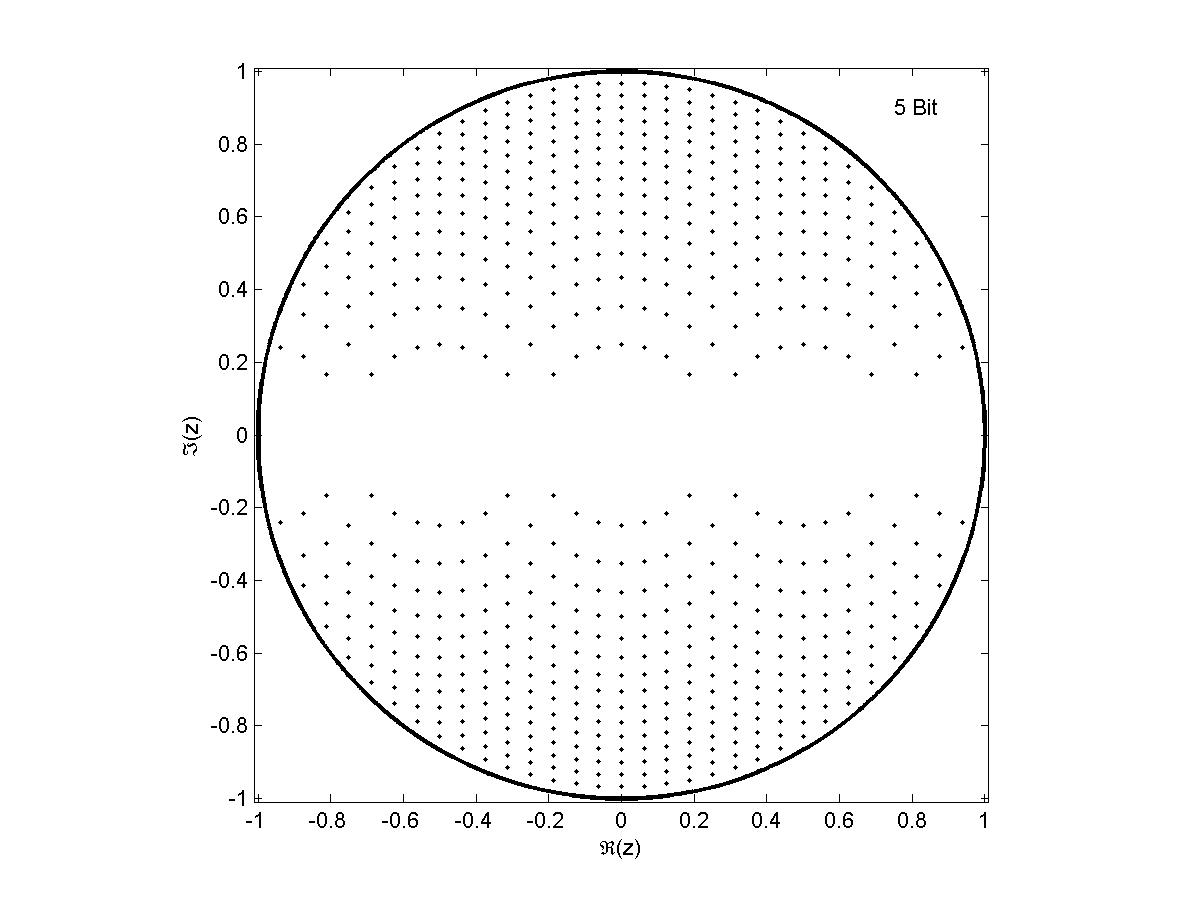
\includegraphics[scale=.35]{graph/QuantPolePlotDirect_1}
					\end{flushright}
				\end{figure}
			}
			\only<3>{
				\begin{figure}
					\begin{flushright}
						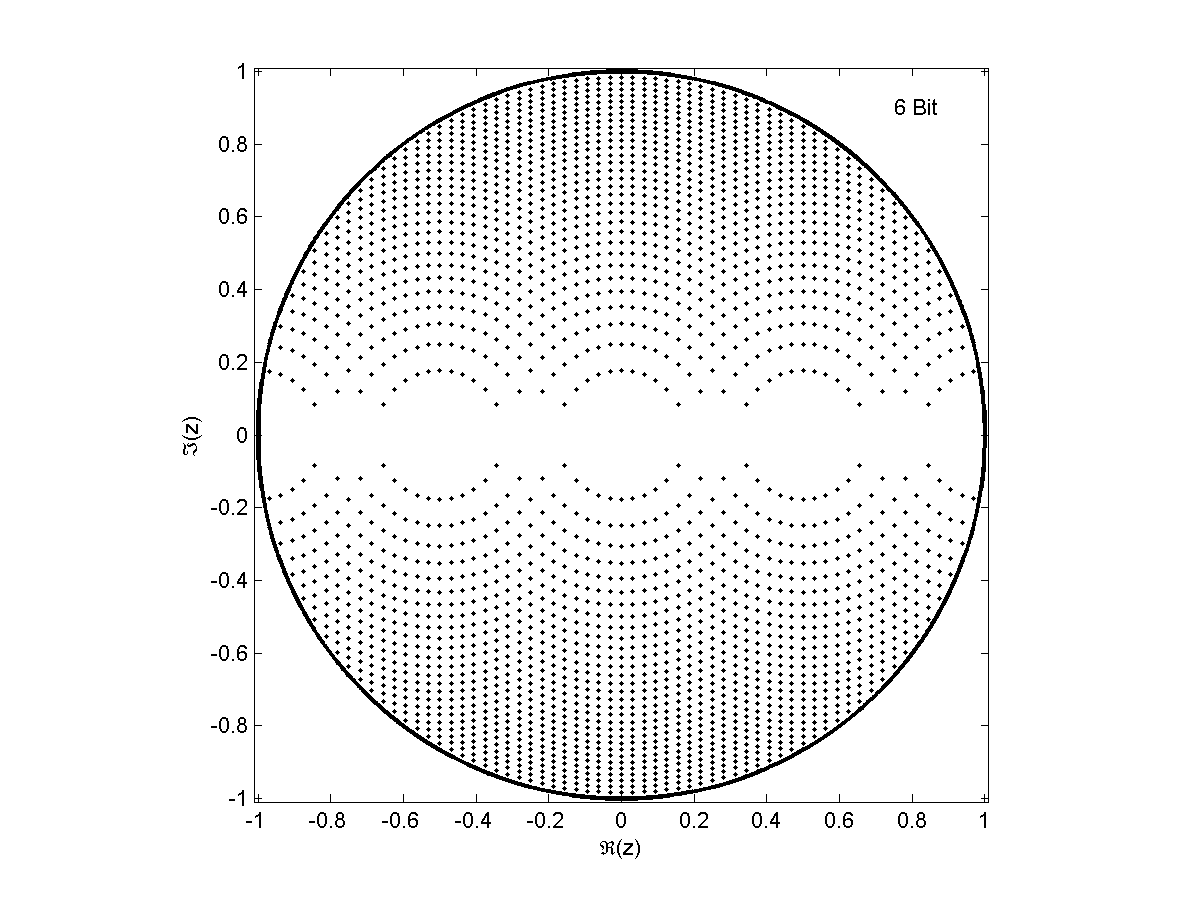
\includegraphics[scale=.35]{graph/QuantPolePlotDirect_2}
					\end{flushright}
				\end{figure}
			}
			\only<4>{
				\begin{figure}
					\begin{flushright}
						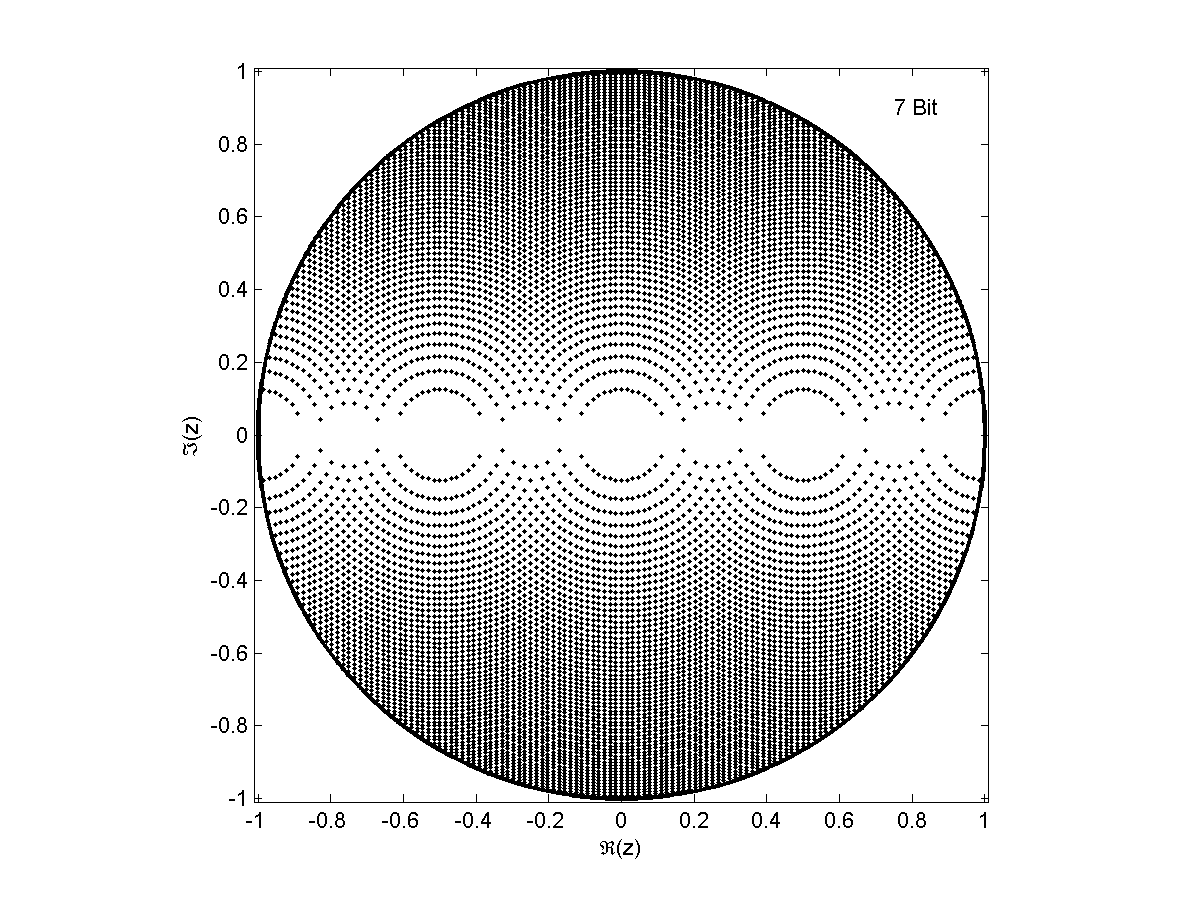
\includegraphics[scale=.35]{graph/QuantPolePlotDirect_3}
					\end{flushright}
				\end{figure}
			}
			\only<5>{
				\begin{figure}
					\begin{flushright}
						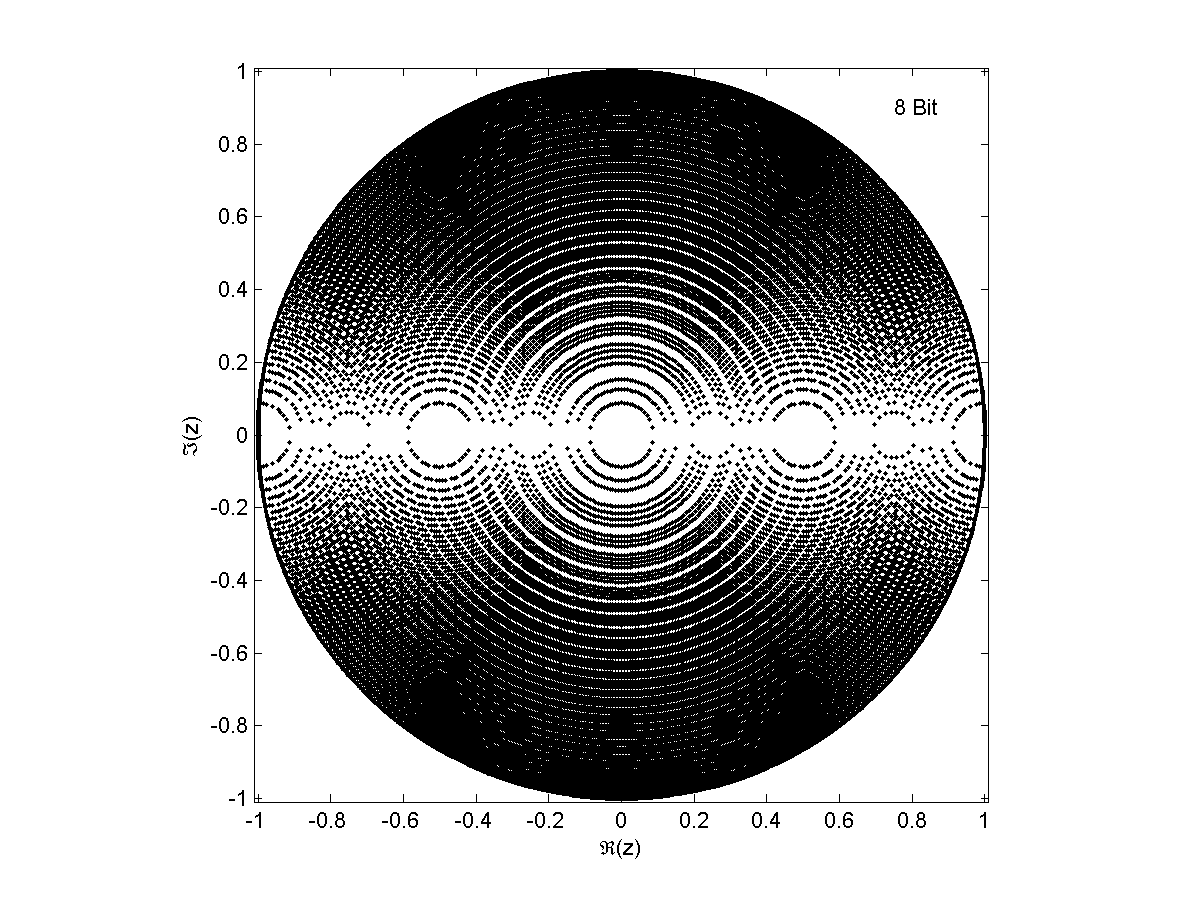
\includegraphics[scale=.35]{graph/QuantPolePlotDirect_4}
					\end{flushright}
				\end{figure}
			}
            \vspace{50mm}
 		\end{frame}
\section{summary}
		\begin{frame}{filter summary}{FIR \& IIR}
            \begin{table}
                \centering
                    \begin{tabular}{l|cc}
                        & \textbf{FIR} & \textbf{IIR}\\
                        \hline
                        IR length & finite & infinite\\
                        structure & non-recursive & recursive\\
                        phase linearity & possible & impossible\\
                        ratio steepness/workload & low & high\\
                        stability & guaranteed & possibly unstable
                    \end{tabular}
            \end{table}
            \bigskip
            \begin{itemize}
                \item   every LTI system is \textbf{completely described} either by
                    \begin{itemize}
                        \item   its complex transfer function,
                        \item   its impulse response, or
                        \item   its pole and zero positions in the z-plane
                    \end{itemize}
            \end{itemize}
 		\end{frame}

\end{document}

